\documentclass[twoside]{book}

% Packages required by doxygen
\usepackage{fixltx2e}
\usepackage{calc}
\usepackage{doxygen}
\usepackage{graphicx}
\usepackage[utf8]{inputenc}
\usepackage{makeidx}
\usepackage{multicol}
\usepackage{multirow}
\PassOptionsToPackage{warn}{textcomp}
\usepackage{textcomp}
\usepackage[nointegrals]{wasysym}
\usepackage[table]{xcolor}

% Font selection
\usepackage[T1]{fontenc}
\usepackage{mathptmx}
\usepackage[scaled=.90]{helvet}
\usepackage{courier}
\usepackage{amssymb}
\usepackage{sectsty}
\renewcommand{\familydefault}{\sfdefault}
\allsectionsfont{%
  \fontseries{bc}\selectfont%
  \color{darkgray}%
}
\renewcommand{\DoxyLabelFont}{%
  \fontseries{bc}\selectfont%
  \color{darkgray}%
}
\newcommand{\+}{\discretionary{\mbox{\scriptsize$\hookleftarrow$}}{}{}}

% Page & text layout
\usepackage{geometry}
\geometry{%
  a4paper,%
  top=2.5cm,%
  bottom=2.5cm,%
  left=2.5cm,%
  right=2.5cm%
}
\tolerance=750
\hfuzz=15pt
\hbadness=750
\setlength{\emergencystretch}{15pt}
\setlength{\parindent}{0cm}
\setlength{\parskip}{0.2cm}
\makeatletter
\renewcommand{\paragraph}{%
  \@startsection{paragraph}{4}{0ex}{-1.0ex}{1.0ex}{%
    \normalfont\normalsize\bfseries\SS@parafont%
  }%
}
\renewcommand{\subparagraph}{%
  \@startsection{subparagraph}{5}{0ex}{-1.0ex}{1.0ex}{%
    \normalfont\normalsize\bfseries\SS@subparafont%
  }%
}
\makeatother

% Headers & footers
\usepackage{fancyhdr}
\pagestyle{fancyplain}
\fancyhead[LE]{\fancyplain{}{\bfseries\thepage}}
\fancyhead[CE]{\fancyplain{}{}}
\fancyhead[RE]{\fancyplain{}{\bfseries\leftmark}}
\fancyhead[LO]{\fancyplain{}{\bfseries\rightmark}}
\fancyhead[CO]{\fancyplain{}{}}
\fancyhead[RO]{\fancyplain{}{\bfseries\thepage}}
\fancyfoot[LE]{\fancyplain{}{}}
\fancyfoot[CE]{\fancyplain{}{}}
\fancyfoot[RE]{\fancyplain{}{\bfseries\scriptsize Generated on Wed Sep 24 2014 01\+:34\+:51 for P\+A04 by Doxygen }}
\fancyfoot[LO]{\fancyplain{}{\bfseries\scriptsize Generated on Wed Sep 24 2014 01\+:34\+:51 for P\+A04 by Doxygen }}
\fancyfoot[CO]{\fancyplain{}{}}
\fancyfoot[RO]{\fancyplain{}{}}
\renewcommand{\footrulewidth}{0.4pt}
\renewcommand{\chaptermark}[1]{%
  \markboth{#1}{}%
}
\renewcommand{\sectionmark}[1]{%
  \markright{\thesection\ #1}%
}

% Indices & bibliography
\usepackage{natbib}
\usepackage[titles]{tocloft}
\setcounter{tocdepth}{3}
\setcounter{secnumdepth}{5}
\makeindex

% Hyperlinks (required, but should be loaded last)
\usepackage{ifpdf}
\ifpdf
  \usepackage[pdftex,pagebackref=true]{hyperref}
\else
  \usepackage[ps2pdf,pagebackref=true]{hyperref}
\fi
\hypersetup{%
  colorlinks=true,%
  linkcolor=blue,%
  citecolor=blue,%
  unicode%
}

% Custom commands
\newcommand{\clearemptydoublepage}{%
  \newpage{\pagestyle{empty}\cleardoublepage}%
}


%===== C O N T E N T S =====

\begin{document}

% Titlepage & ToC
\hypersetup{pageanchor=false,
             bookmarks=true,
             bookmarksnumbered=true,
             pdfencoding=unicode
            }
\pagenumbering{roman}
\begin{titlepage}
\vspace*{7cm}
\begin{center}%
{\Large P\+A04 }\\
\vspace*{1cm}
{\large Generated by Doxygen 1.8.8}\\
\vspace*{0.5cm}
{\small Wed Sep 24 2014 01:34:51}\\
\end{center}
\end{titlepage}
\clearemptydoublepage
\tableofcontents
\clearemptydoublepage
\pagenumbering{arabic}
\hypersetup{pageanchor=true}

%--- Begin generated contents ---
\chapter{Hierarchical Index}
\section{Class Hierarchy}
This inheritance list is sorted roughly, but not completely, alphabetically\+:\begin{DoxyCompactList}
\item \contentsline{section}{Queue$<$ Data\+Type $>$}{\pageref{class_queue}}{}
\begin{DoxyCompactList}
\item \contentsline{section}{Queue\+Array$<$ Data\+Type $>$}{\pageref{class_queue_array}}{}
\item \contentsline{section}{Queue\+Linked$<$ Data\+Type $>$}{\pageref{class_queue_linked}}{}
\end{DoxyCompactList}
\end{DoxyCompactList}

\chapter{Class Index}
\section{Class List}
Here are the classes, structs, unions and interfaces with brief descriptions\+:\begin{DoxyCompactList}
\item\contentsline{section}{\hyperlink{class_greater}{Greater$<$ Key\+Type $>$} }{\pageref{class_greater}}{}
\item\contentsline{section}{\hyperlink{class_heap}{Heap$<$ Data\+Type, Key\+Type, Comparator $>$} }{\pageref{class_heap}}{}
\item\contentsline{section}{\hyperlink{class_less}{Less$<$ Key\+Type $>$} }{\pageref{class_less}}{}
\item\contentsline{section}{\hyperlink{class_priority_queue}{Priority\+Queue$<$ Data\+Type, Key\+Type, Comparator $>$} }{\pageref{class_priority_queue}}{}
\item\contentsline{section}{\hyperlink{struct_task_data}{Task\+Data} }{\pageref{struct_task_data}}{}
\item\contentsline{section}{\hyperlink{class_test_data}{Test\+Data} }{\pageref{class_test_data}}{}
\item\contentsline{section}{\hyperlink{class_test_data_item}{Test\+Data\+Item$<$ Key\+Type $>$} }{\pageref{class_test_data_item}}{}
\end{DoxyCompactList}

\chapter{File Index}
\section{File List}
Here is a list of all documented files with brief descriptions\+:\begin{DoxyCompactList}
\item\contentsline{section}{\hyperlink{_b_s_tree_8cpp}{B\+S\+Tree.\+cpp} \\*This program will implement a Binary Search Tree }{\pageref{_b_s_tree_8cpp}}{}
\item\contentsline{section}{{\bfseries B\+S\+Tree.\+h} }{\pageref{_b_s_tree_8h}}{}
\item\contentsline{section}{\hyperlink{_hash_table_8cpp}{Hash\+Table.\+cpp} \\*This program will implement a Hash Table }{\pageref{_hash_table_8cpp}}{}
\item\contentsline{section}{{\bfseries Hash\+Table.\+h} }{\pageref{_hash_table_8h}}{}
\item\contentsline{section}{\hyperlink{login_8cpp}{login.\+cpp} \\*This program will implement the Exercise 1 of Lab 10 Hash Table }{\pageref{login_8cpp}}{}
\end{DoxyCompactList}

\chapter{Class Documentation}
\hypertarget{classbinary_search}{\section{binary\+Search Class Reference}
\label{classbinary_search}\index{binary\+Search@{binary\+Search}}
}
Inheritance diagram for binary\+Search\+:\begin{figure}[H]
\begin{center}
\leavevmode
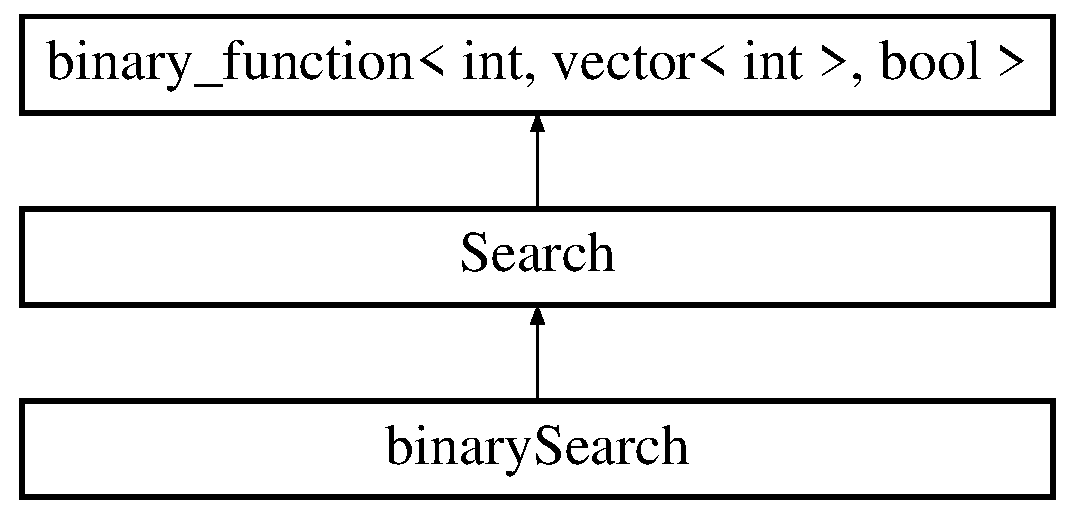
\includegraphics[height=3.000000cm]{classbinary_search}
\end{center}
\end{figure}
\subsection*{Public Member Functions}
\begin{DoxyCompactItemize}
\item 
\hypertarget{classbinary_search_a8e145edfb29183d7e1b265bd4cf4293f}{bool {\bfseries operator()} (int search\+Value, const vector$<$ int $>$ \&keys) const }\label{classbinary_search_a8e145edfb29183d7e1b265bd4cf4293f}

\end{DoxyCompactItemize}


The documentation for this class was generated from the following file\+:\begin{DoxyCompactItemize}
\item 
search.\+cpp\end{DoxyCompactItemize}

\hypertarget{classlinear_search}{\section{linear\+Search Class Reference}
\label{classlinear_search}\index{linear\+Search@{linear\+Search}}
}
Inheritance diagram for linear\+Search\+:\begin{figure}[H]
\begin{center}
\leavevmode
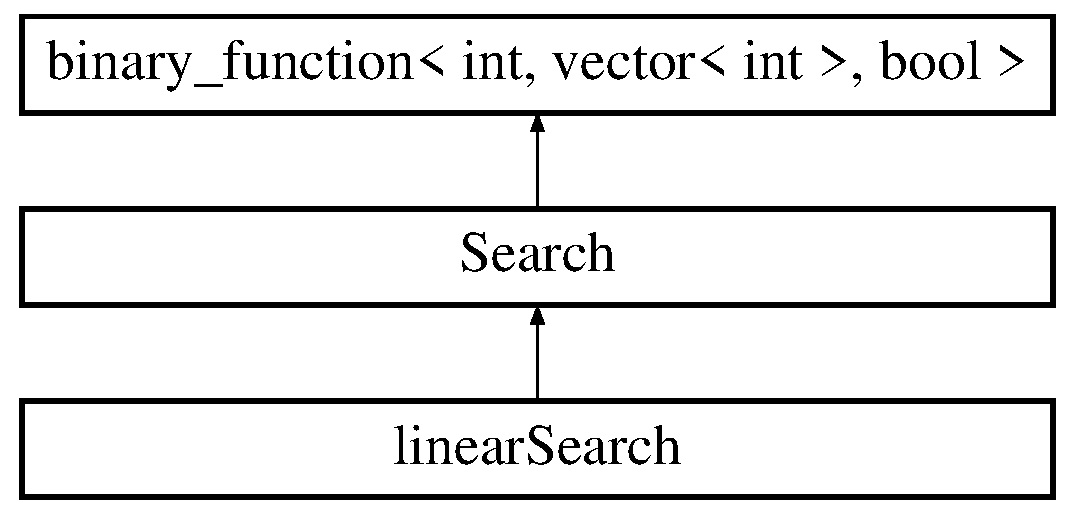
\includegraphics[height=3.000000cm]{classlinear_search}
\end{center}
\end{figure}
\subsection*{Public Member Functions}
\begin{DoxyCompactItemize}
\item 
\hypertarget{classlinear_search_a447bc4f724457f1786dc36c10626bfa8}{bool {\bfseries operator()} (int search\+Value, const vector$<$ int $>$ \&keys) const }\label{classlinear_search_a447bc4f724457f1786dc36c10626bfa8}

\end{DoxyCompactItemize}


The documentation for this class was generated from the following file\+:\begin{DoxyCompactItemize}
\item 
search.\+cpp\end{DoxyCompactItemize}

\hypertarget{class_search}{\section{Search Class Reference}
\label{class_search}\index{Search@{Search}}
}
Inheritance diagram for Search\+:\begin{figure}[H]
\begin{center}
\leavevmode
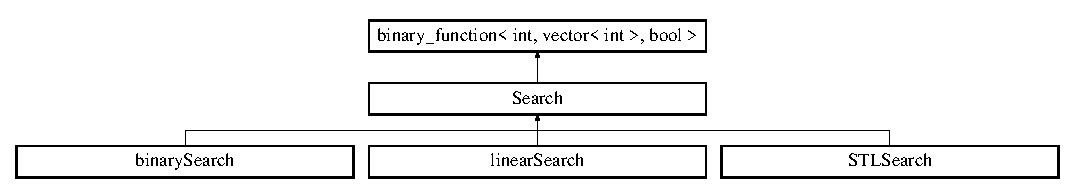
\includegraphics[height=2.153846cm]{class_search}
\end{center}
\end{figure}


The documentation for this class was generated from the following file\+:\begin{DoxyCompactItemize}
\item 
search.\+cpp\end{DoxyCompactItemize}

\hypertarget{class_s_t_l_search}{\section{S\+T\+L\+Search Class Reference}
\label{class_s_t_l_search}\index{S\+T\+L\+Search@{S\+T\+L\+Search}}
}
Inheritance diagram for S\+T\+L\+Search\+:\begin{figure}[H]
\begin{center}
\leavevmode
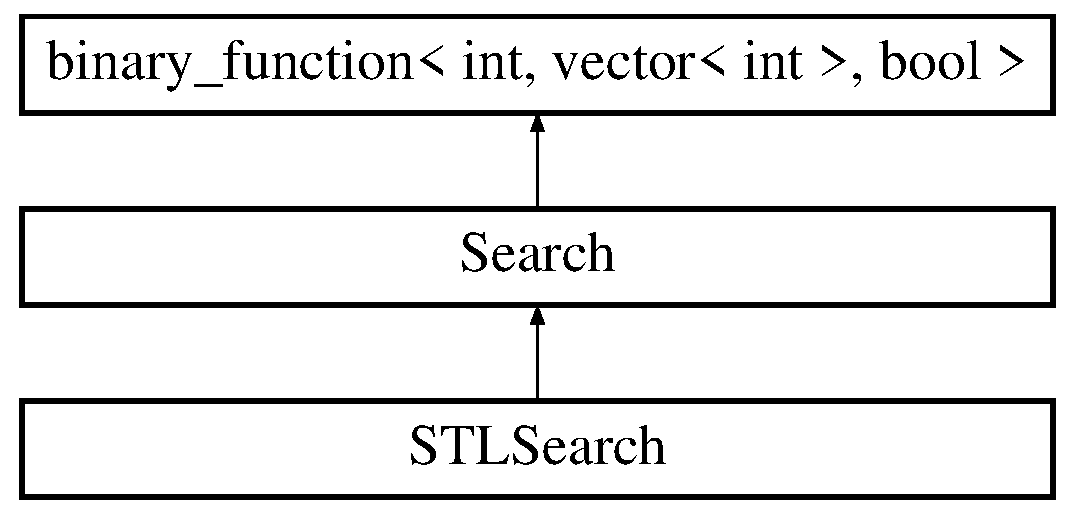
\includegraphics[height=3.000000cm]{class_s_t_l_search}
\end{center}
\end{figure}
\subsection*{Public Member Functions}
\begin{DoxyCompactItemize}
\item 
\hypertarget{class_s_t_l_search_a0f3684e33bd5e47317ab5a94d6f52dba}{bool {\bfseries operator()} (int search\+Value, const vector$<$ int $>$ \&keys) const }\label{class_s_t_l_search_a0f3684e33bd5e47317ab5a94d6f52dba}

\end{DoxyCompactItemize}


The documentation for this class was generated from the following file\+:\begin{DoxyCompactItemize}
\item 
search.\+cpp\end{DoxyCompactItemize}

\hypertarget{class_test_vector}{\section{Test\+Vector Class Reference}
\label{class_test_vector}\index{Test\+Vector@{Test\+Vector}}
}
\subsection*{Public Member Functions}
\begin{DoxyCompactItemize}
\item 
\hypertarget{class_test_vector_abf540180761043bb7ac2665e147bdd33}{{\bfseries Test\+Vector} (int size)}\label{class_test_vector_abf540180761043bb7ac2665e147bdd33}

\item 
\hypertarget{class_test_vector_a4a48046f67cc822ce9a6907f022a5d61}{{\bfseries Test\+Vector} (const \hyperlink{class_test_vector}{Test\+Vector} \&rhs)}\label{class_test_vector_a4a48046f67cc822ce9a6907f022a5d61}

\item 
\hypertarget{class_test_vector_a8d4a95de7e0e9985ffcd86280efb631d}{\hyperlink{class_test_vector}{Test\+Vector} \& {\bfseries operator++} ()}\label{class_test_vector_a8d4a95de7e0e9985ffcd86280efb631d}

\item 
\hypertarget{class_test_vector_a1b9640623055cd4618606cd2f0ed08b3}{\hyperlink{class_test_vector}{Test\+Vector} {\bfseries operator++} (int ignored)}\label{class_test_vector_a1b9640623055cd4618606cd2f0ed08b3}

\item 
\hypertarget{class_test_vector_ae244371b88cb0ab127a877e5206b7ed8}{int {\bfseries operator\mbox{[}$\,$\mbox{]}} (int loc) const }\label{class_test_vector_ae244371b88cb0ab127a877e5206b7ed8}

\end{DoxyCompactItemize}


The documentation for this class was generated from the following files\+:\begin{DoxyCompactItemize}
\item 
Test\+Vector.\+h\item 
Test\+Vector.\+cpp\end{DoxyCompactItemize}

\hypertarget{class_timer}{\section{Timer Class Reference}
\label{class_timer}\index{Timer@{Timer}}
}
\subsection*{Public Member Functions}
\begin{DoxyCompactItemize}
\item 
\hyperlink{class_timer_a5f16e8da27d2a5a5242dead46de05d97}{Timer} ()
\item 
void \hyperlink{class_timer_a3a8b5272198d029779dc9302a54305a8}{start} ()  throw (runtime\+\_\+error)
\item 
void \hyperlink{class_timer_a63f0eb44b27402196590a03781515dba}{stop} ()  throw (logic\+\_\+error)
\item 
double \hyperlink{class_timer_ad306e18f8d8a0296e001683f92d7f86e}{get\+Elapsed\+Time} () const   throw (logic\+\_\+error)
\end{DoxyCompactItemize}


\subsection{Constructor \& Destructor Documentation}
\hypertarget{class_timer_a5f16e8da27d2a5a5242dead46de05d97}{\index{Timer@{Timer}!Timer@{Timer}}
\index{Timer@{Timer}!Timer@{Timer}}
\subsubsection[{Timer}]{\setlength{\rightskip}{0pt plus 5cm}Timer\+::\+Timer (
\begin{DoxyParamCaption}
{}
\end{DoxyParamCaption}
)}}\label{class_timer_a5f16e8da27d2a5a5242dead46de05d97}
Method implementation Initialize \hyperlink{class_timer}{Timer} object


\begin{DoxyParams}{Parameters}
{\em none} & \\
\hline
\end{DoxyParams}
\begin{DoxyReturn}{Returns}
none 
\end{DoxyReturn}
\begin{DoxyPrecond}{Precondition}
None 
\end{DoxyPrecond}
\begin{DoxyPostcond}{Postcondition}
Initialize the internal timer valuesso that the timer is ready to measure time 
\end{DoxyPostcond}


\subsection{Member Function Documentation}
\hypertarget{class_timer_ad306e18f8d8a0296e001683f92d7f86e}{\index{Timer@{Timer}!get\+Elapsed\+Time@{get\+Elapsed\+Time}}
\index{get\+Elapsed\+Time@{get\+Elapsed\+Time}!Timer@{Timer}}
\subsubsection[{get\+Elapsed\+Time}]{\setlength{\rightskip}{0pt plus 5cm}double Timer\+::get\+Elapsed\+Time (
\begin{DoxyParamCaption}
{}
\end{DoxyParamCaption}
) const throw  logic\+\_\+error) }}\label{class_timer_ad306e18f8d8a0296e001683f92d7f86e}
Find how much time has elapsed between start and end of timer


\begin{DoxyParams}{Parameters}
{\em none} & \\
\hline
\end{DoxyParams}
\begin{DoxyReturn}{Returns}
double Length of time interval in seconds 
\end{DoxyReturn}
\begin{DoxyPrecond}{Precondition}
\hyperlink{class_timer}{Timer} has been started and ended 
\end{DoxyPrecond}
\begin{DoxyPostcond}{Postcondition}
Returns the length of the time interval in seconds 
\end{DoxyPostcond}
\hypertarget{class_timer_a3a8b5272198d029779dc9302a54305a8}{\index{Timer@{Timer}!start@{start}}
\index{start@{start}!Timer@{Timer}}
\subsubsection[{start}]{\setlength{\rightskip}{0pt plus 5cm}void Timer\+::start (
\begin{DoxyParamCaption}
{}
\end{DoxyParamCaption}
) throw  runtime\+\_\+error) }}\label{class_timer_a3a8b5272198d029779dc9302a54305a8}
Set timer started to true and record the beginning time


\begin{DoxyParams}{Parameters}
{\em none} & \\
\hline
\end{DoxyParams}
\begin{DoxyReturn}{Returns}
none 
\end{DoxyReturn}
\begin{DoxyPrecond}{Precondition}
\hyperlink{class_timer}{Timer} has not started yet 
\end{DoxyPrecond}
\begin{DoxyPostcond}{Postcondition}
Mark the beginning of a time interval; start the timer 
\end{DoxyPostcond}
\hypertarget{class_timer_a63f0eb44b27402196590a03781515dba}{\index{Timer@{Timer}!stop@{stop}}
\index{stop@{stop}!Timer@{Timer}}
\subsubsection[{stop}]{\setlength{\rightskip}{0pt plus 5cm}void Timer\+::stop (
\begin{DoxyParamCaption}
{}
\end{DoxyParamCaption}
) throw  logic\+\_\+error) }}\label{class_timer_a63f0eb44b27402196590a03781515dba}
Set timer started to false and record end time of timer


\begin{DoxyParams}{Parameters}
{\em none} & \\
\hline
\end{DoxyParams}
\begin{DoxyReturn}{Returns}
none 
\end{DoxyReturn}
\begin{DoxyPrecond}{Precondition}
\hyperlink{class_timer}{Timer} has started 
\end{DoxyPrecond}
\begin{DoxyPostcond}{Postcondition}
Marks the end of a time interval; stop the timer 
\end{DoxyPostcond}


The documentation for this class was generated from the following files\+:\begin{DoxyCompactItemize}
\item 
Timer.\+h\item 
\hyperlink{_timer_8cpp}{Timer.\+cpp}\item 
Timer.\+cs\end{DoxyCompactItemize}

\chapter{File Documentation}
\hypertarget{_timer_8cpp}{\section{Timer.\+cpp File Reference}
\label{_timer_8cpp}\index{Timer.\+cpp@{Timer.\+cpp}}
}


This program implements a stopwatch. It starts, stops and stores the time elapsed in between.  


{\ttfamily \#include $<$sys/time.\+h$>$}\\*
{\ttfamily \#include $<$stdexcept$>$}\\*
{\ttfamily \#include $<$iostream$>$}\\*
{\ttfamily \#include \char`\"{}Timer.\+h\char`\"{}}\\*


\subsection{Detailed Description}
This program implements a stopwatch. It starts, stops and stores the time elapsed in between. 

\begin{DoxyAuthor}{Author}
Tim Kwist 
\end{DoxyAuthor}
\begin{DoxyVersion}{Version}
1.\+0 
\end{DoxyVersion}
\begin{DoxyDate}{Date}
Wednesday, September 23nd, 2014
\end{DoxyDate}
The program uses system time to determine elapsed time. Starting stores the current system time. Stopping gets the current system time and subtracts the beginning time to get the elapsed time. 
%--- End generated contents ---

% Index
\newpage
\phantomsection
\addcontentsline{toc}{chapter}{Index}
\printindex

\end{document}
